%%% MORITZ 10' %%%

\section{Spinpräzession}
\subsection{Grundlagen}
\begin{frame}
\frametitle{Grundlagen: Spinpräzession}

\begin{itemize}
  \item Spinpräzession von Atomen im Magnetfeld $B$ mit Frequenz $f$
\end{itemize}


\begin{equation*}
    f=\frac{g_\text{F} \cdot \mu_\text{B}}{h} \cdot B = \alpha \cdot B
\end{equation*}
  
  
\begin{equation*}
    \alpha = 4.665\,\text{kHz } \text{\textmu T}^{-1}
\end{equation*}

\end{frame}

\subsection{Aufbau}
\begin{frame}
\frametitle{Aufbau: Spinpräzession}

\setbeamerfont{myfont}{size*=80}
\usebeamerfont{myfont}
\begin{figure}
    \centering
    \def\svgwidth{\textwidth}
    \input{../img/aufbauspinpraez.pdf_tex}
    \caption{Aufbau zur Messung der Spinpräzession.}
\end{figure}
\usebeamerfont{standard}

\begin{itemize}
  \item \textbf{Spule 1:} Kompensation von horizontalem Erdmagnetfeld
  \item \textbf{Spule 4:} Kompensation von vertikalem Erdmagnetfeld
  \item \textbf{Spule 5:} Ein- und Ausschalten von Magnetfeld mit 50\,Hz
\end{itemize}

\end{frame}

\subsection{Auswertung}

\begin{frame}
\frametitle{Auswertung: Spinpräzession}

\begin{figure}
    \centering
    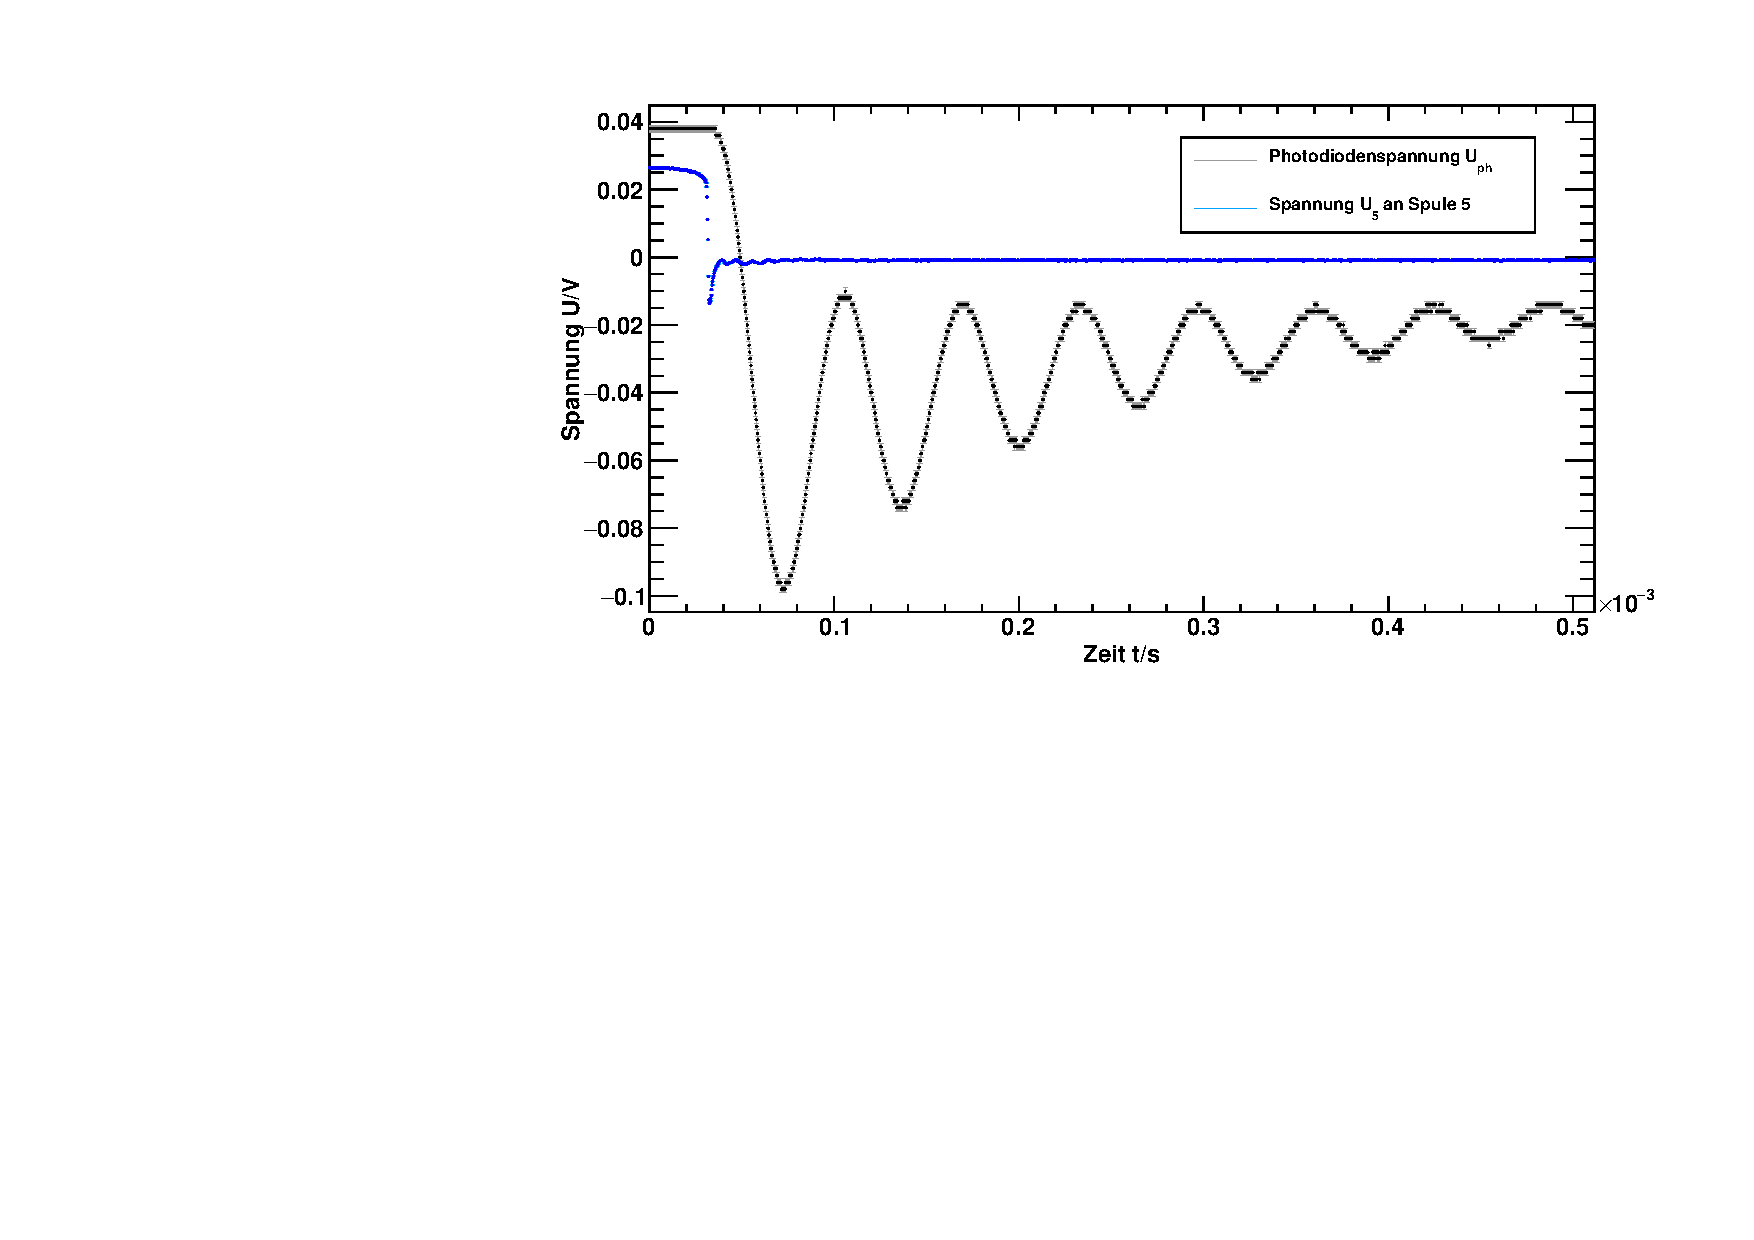
\includegraphics[width=\textwidth]{../img/02-63-7mA-087mA.pdf}
    \caption{Spinpräzession im schwachen Magnetfeld.}  
\end{figure} 
  
\end{frame}


\begin{frame}
\frametitle{Auswertung: Spinpräzession}

\begin{figure}
    \centering
    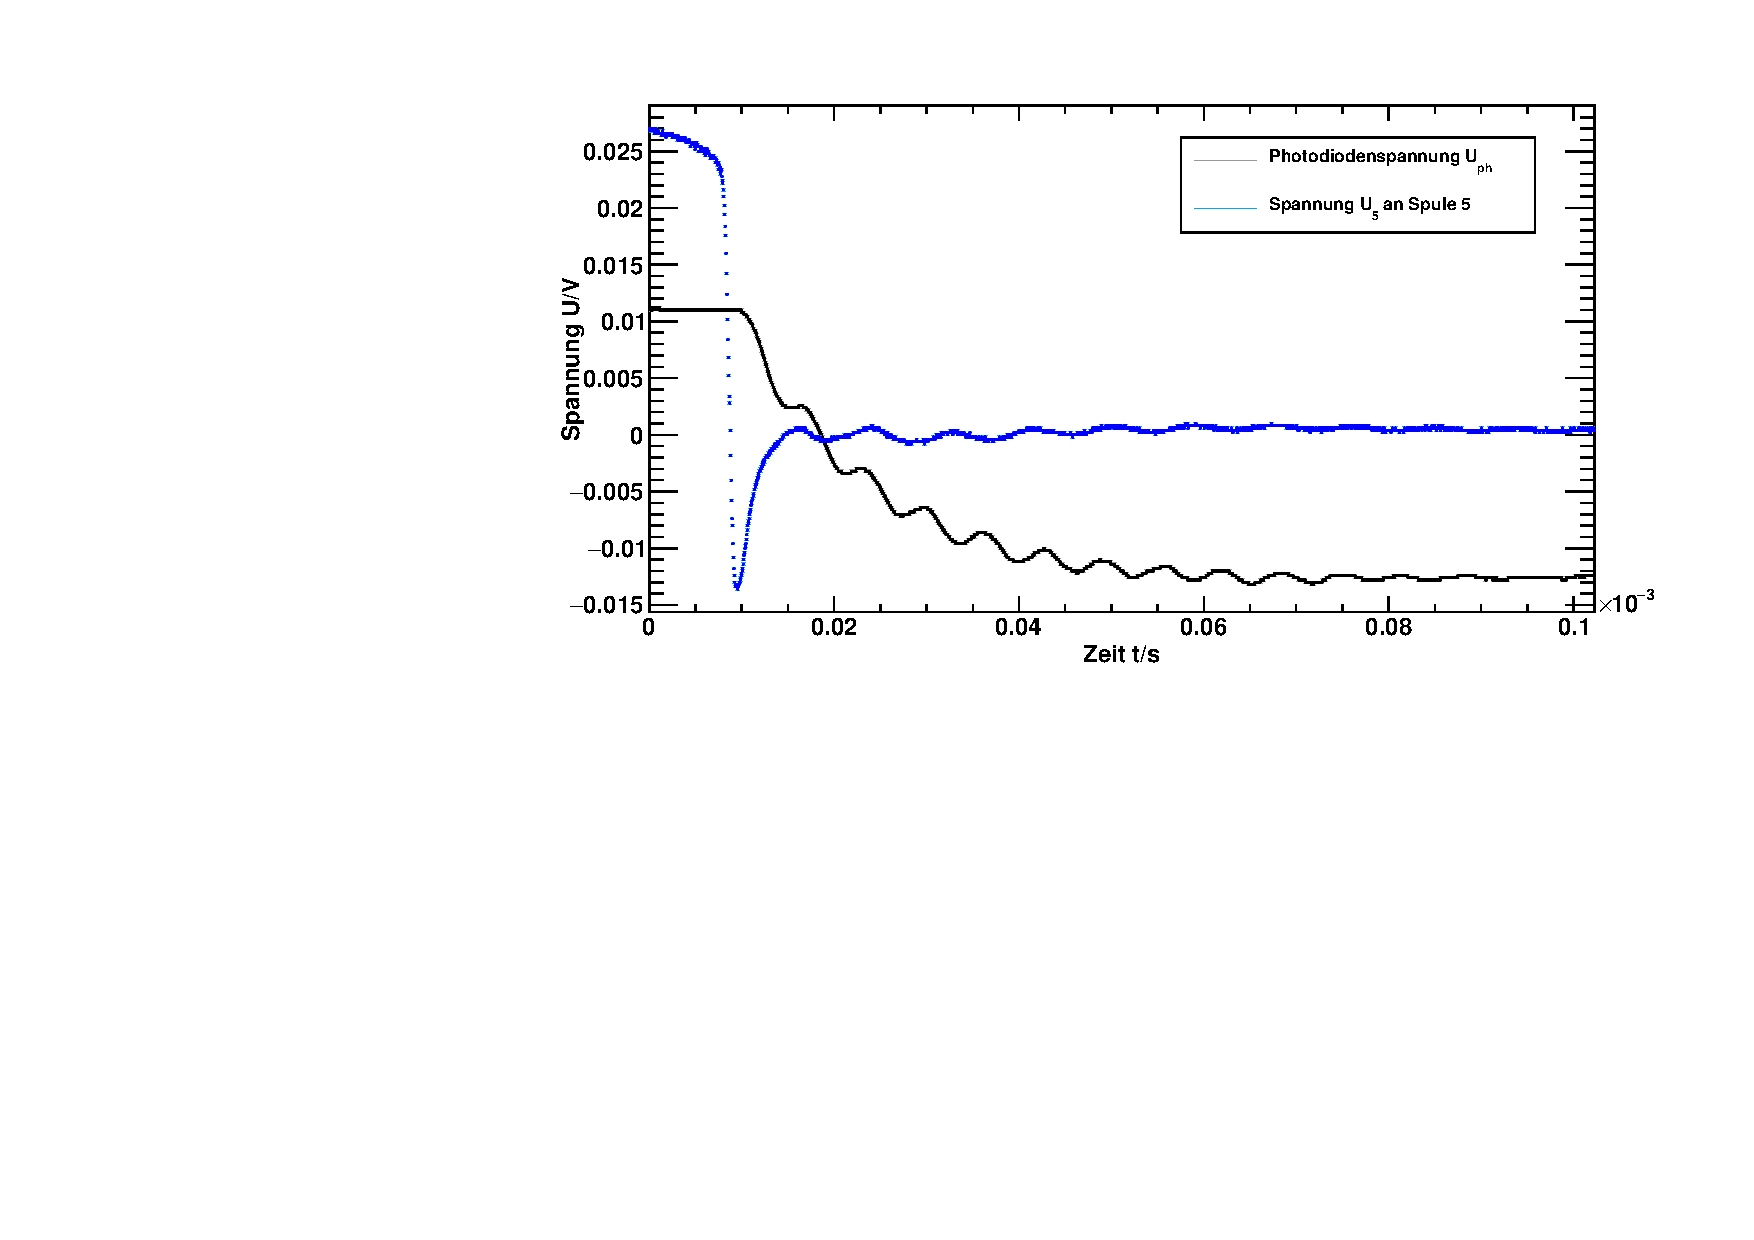
\includegraphics[width=\textwidth]{../img/02-63-7mA-020mA.pdf}
    \caption{Spinpräzession im starken Magnetfeld.}  
\end{figure} 
  
\end{frame}



\begin{frame}
\frametitle{Auswertung: Spinpräzession}

\begin{figure}
    \centering
    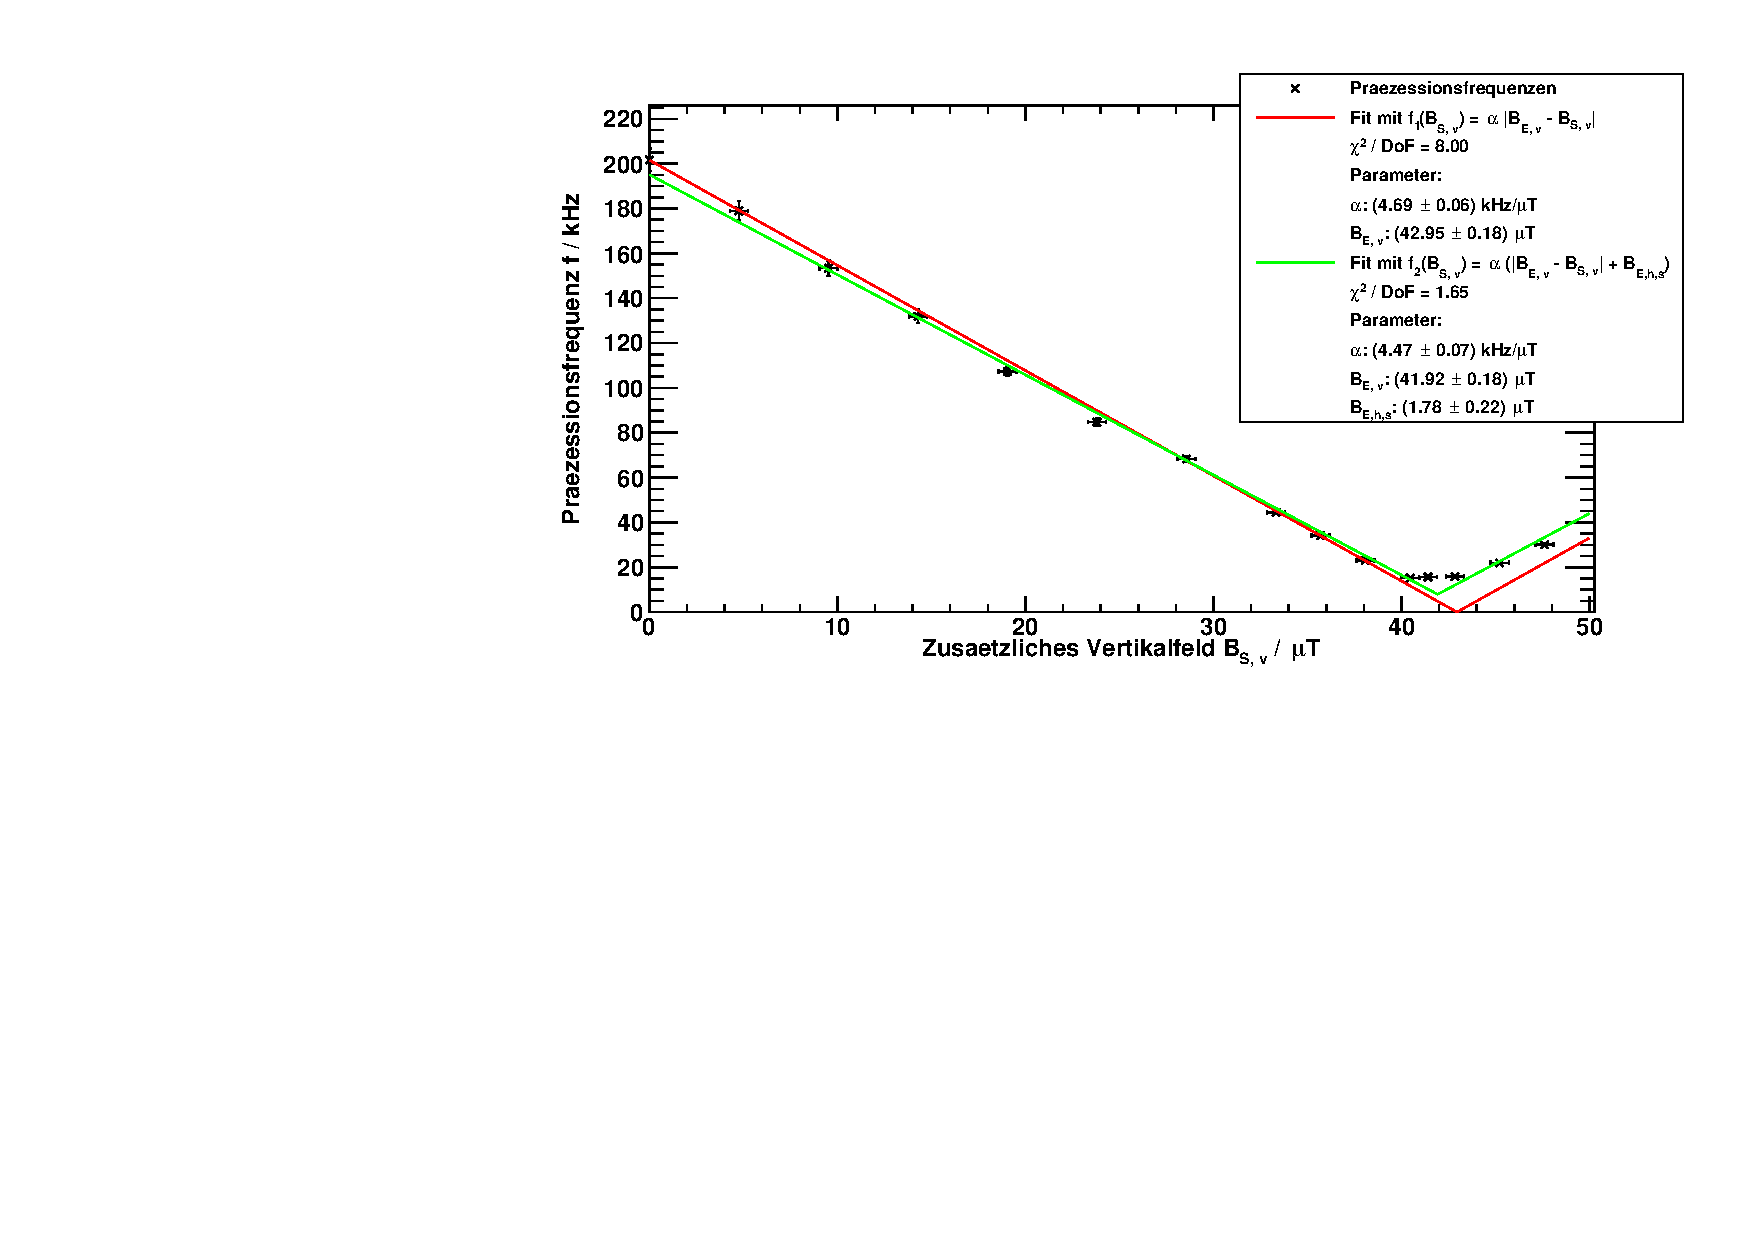
\includegraphics[width=\textwidth]{../img/Rb85.pdf}
    \caption{Magnetfeldabhängigkeit der Spinpräzessionsfrequenz.}  
\end{figure} 
  
\end{frame}


\begin{frame}
\frametitle{Auswertung: Spinpräzession}

Horizontalkomponente des Erdmagnetfelds war nicht vollständig kompensierbar
$\to$ Berechnung der Winkelabweichung des Messaufbaus von der Nordrichtung
\begin{equation*}
    \varphi = \arctan\left( \frac{B_\text{h,s}}{B_\text{h,p}} \right)
    = (8.3 \pm 1.0)^\circ
\end{equation*}

\setbeamerfont{myfont}{size*=80}
\usebeamerfont{myfont}
\begin{figure}
    \centering
    \def\svgwidth{0.5\textwidth}
    \input{../img/arctangans.pdf_tex}
    \caption{Horizontalkomponenten des Erdmagnetfelds senkrecht und parallel zur Strahlrichtung.}
\end{figure}
\usebeamerfont{standard}
  
\end{frame}

\begin{frame}
\frametitle{Auswertung: Spinpräzession}

\begin{figure}
    \centering
    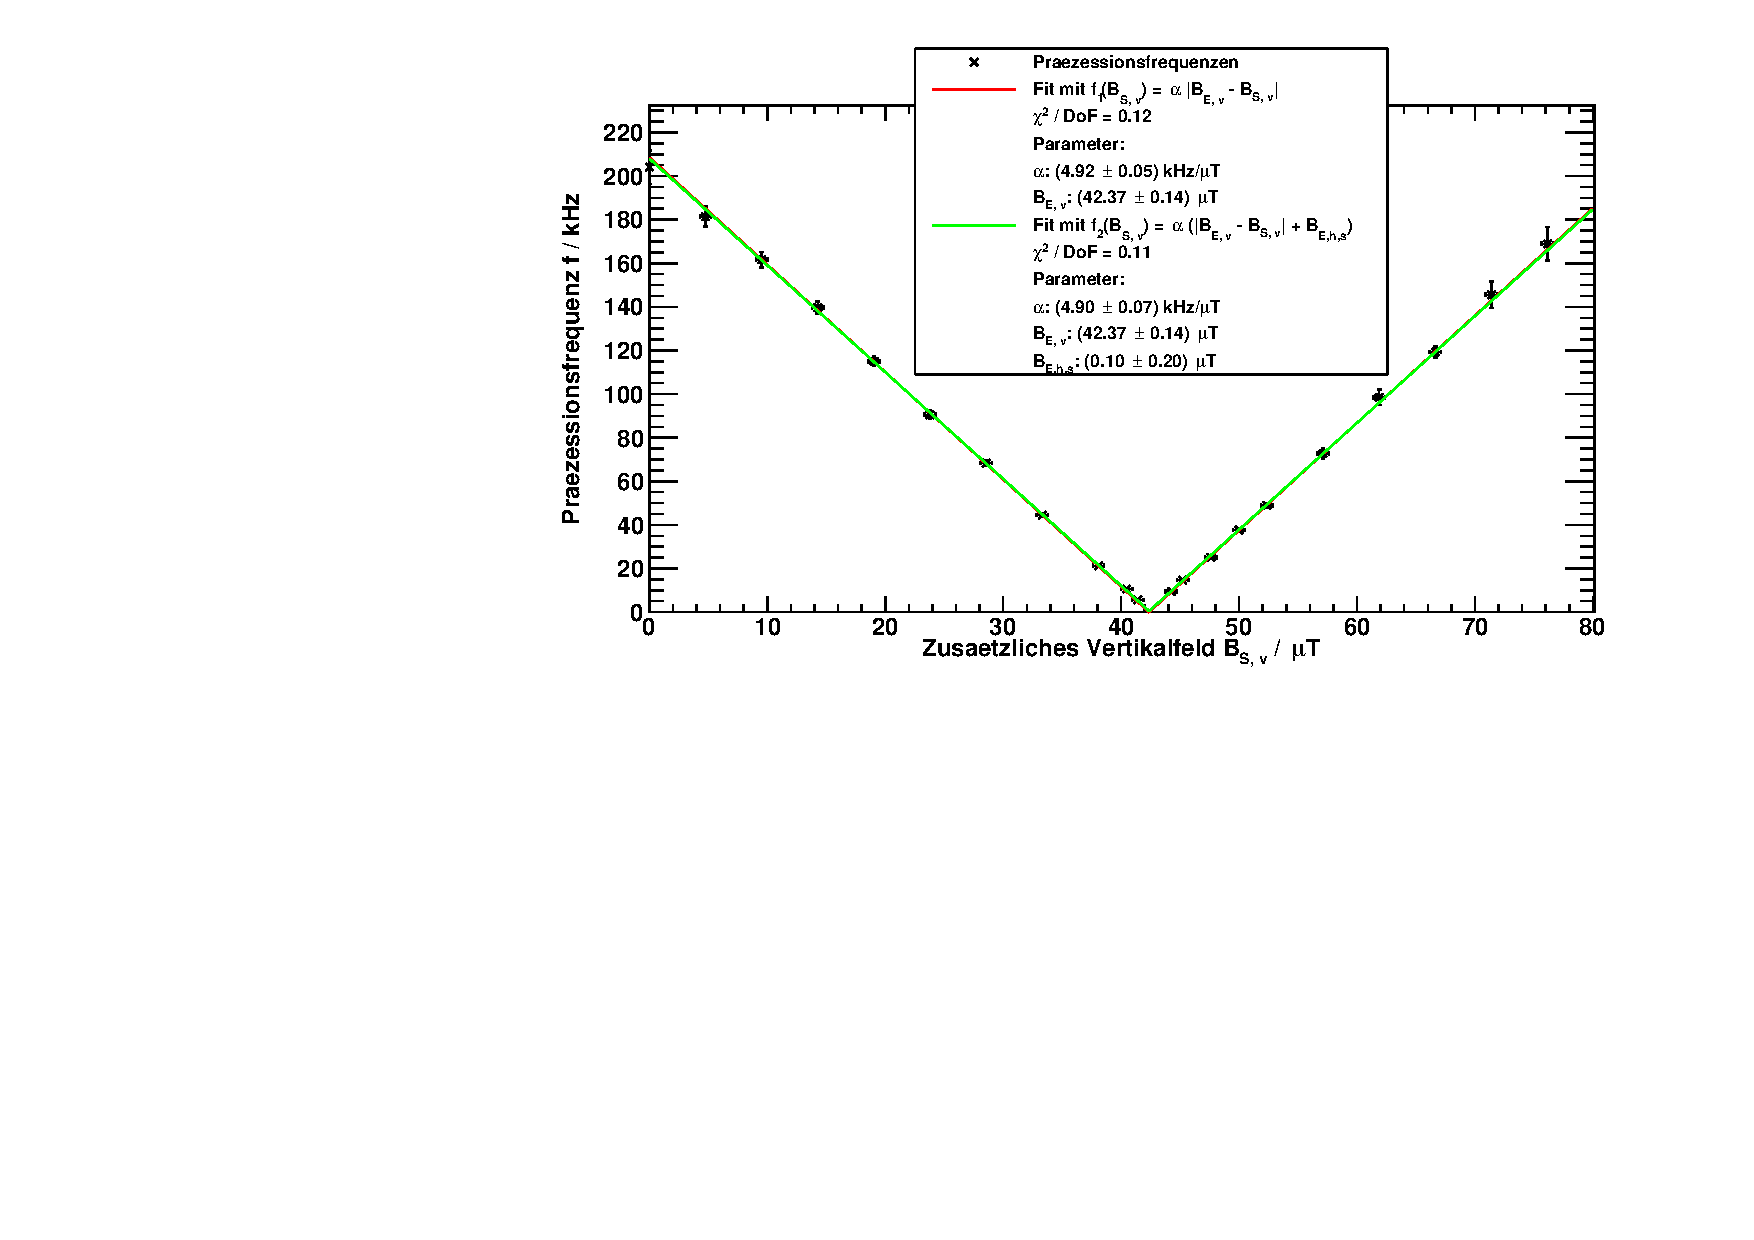
\includegraphics[width=\textwidth]{../img/Rb85_gedreht.pdf}
    \caption{Magnetfeldabhängigkeit der Spinpräzessionsfrequenz nach Ausrichtung des Versuchsaufbaus nach Norden.}  
\end{figure} 
  
\end{frame}




\begin{frame}
\frametitle{Auswertung: Spinpräzession}

\begin{figure}
    \centering
    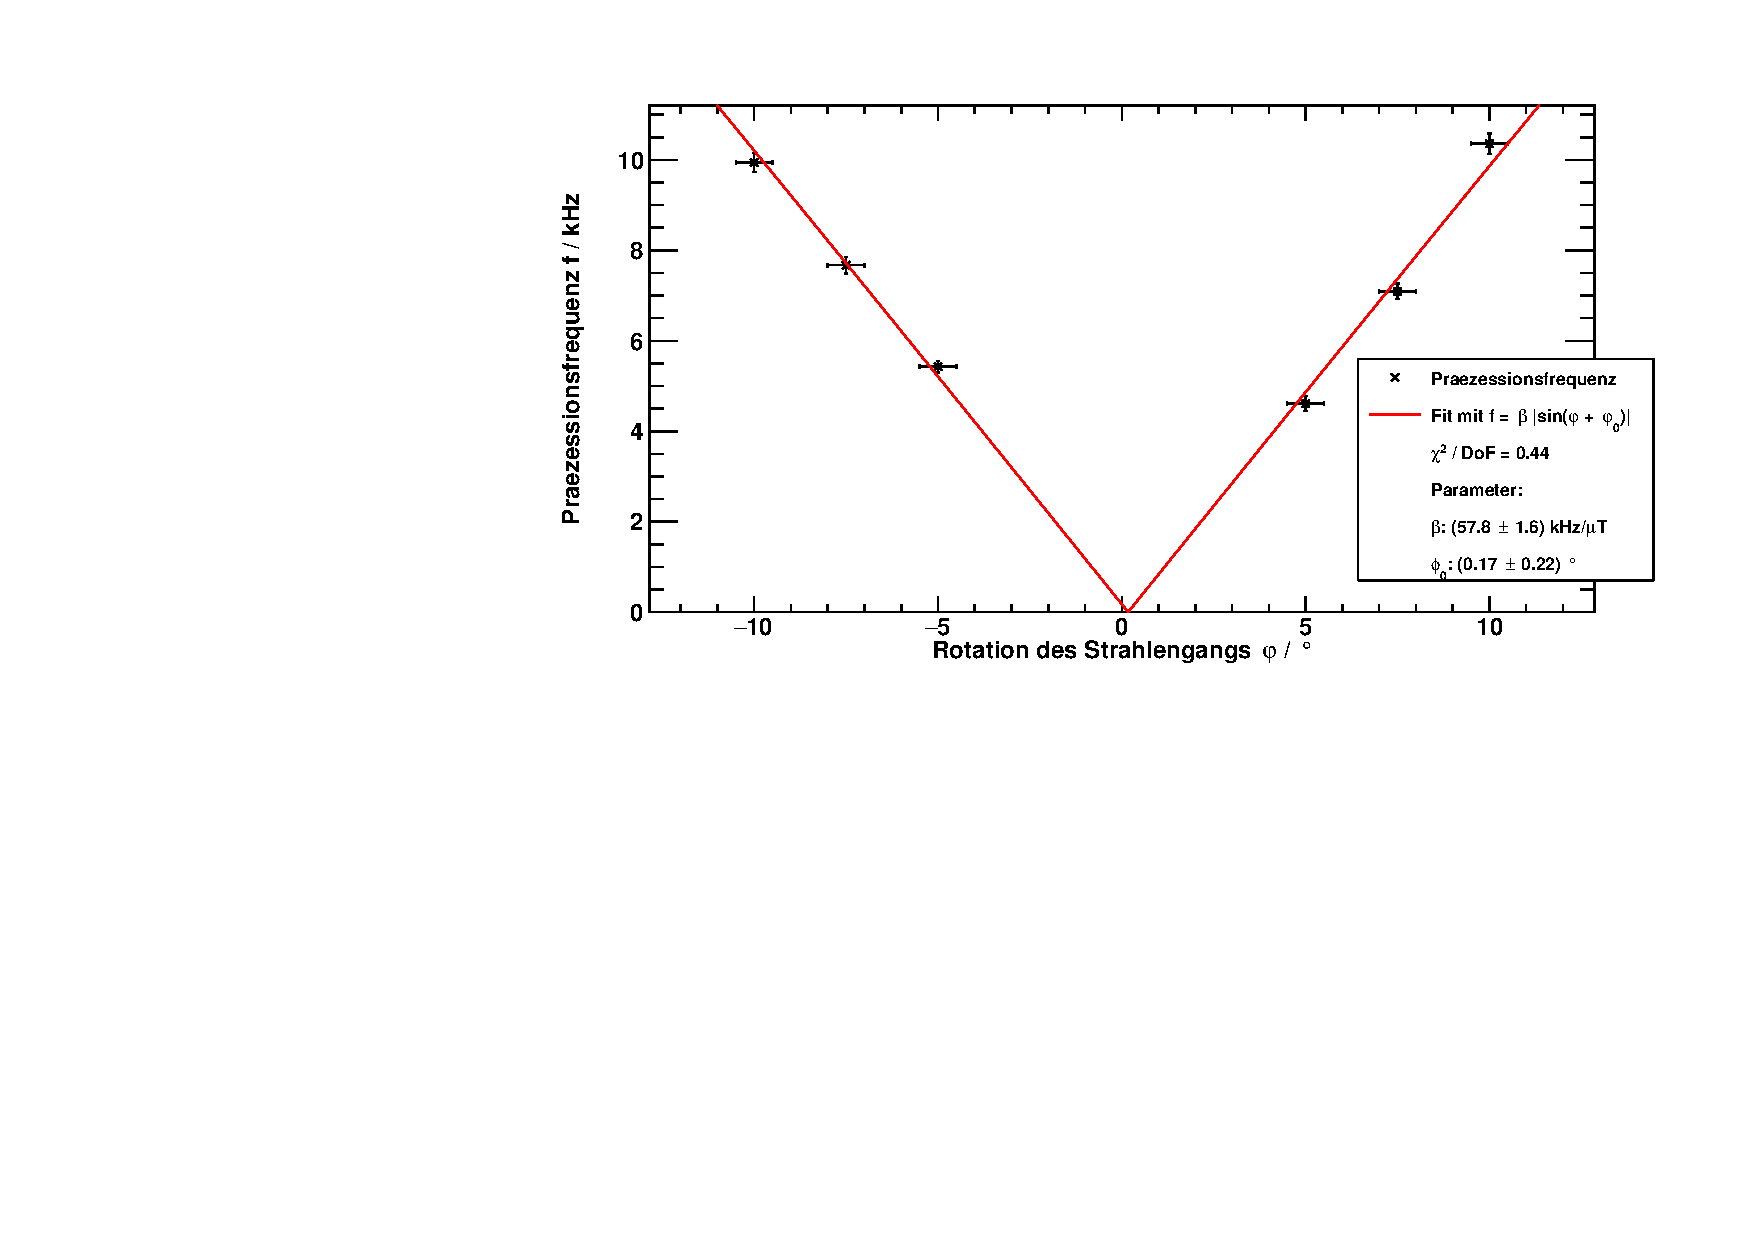
\includegraphics[width=\textwidth]{../img/winkel.pdf}
    \caption{Winkelabhängigkeit der Spinpräzessionsfrequenz.}  
\end{figure} 
  
\end{frame}

\begin{frame}
\frametitle{Ergebnis: Spinpräzession}
\begin{itemize}
    \item Zusammenhang zwischen Magnetfeld und Frequenz
    \begin{equation*}
        \alpha^\text{exp} = 4.92 \pm 0.05\,\text{kHz } \text{\textmu T}^{-1}
    \end{equation*}
    \item Literaturwert
    \begin{equation*}
        \alpha^\text{theo} = 4.665\,\text{kHz } \text{\textmu T}^{-1}
    \end{equation*}
    \item Abweichung durch Umrechnung von Spulenstrom in Magnetfeldstärke?
\end{itemize}
  
\end{frame}
